
\chapter{موارد کاربرد}


\section{تعریف کنش‌گر‌ها}


\begin{table}[h]
	\setlength\extrarowheight{-5pt}
	\centering
	\begin{tabular}{|p{0.05\linewidth}|p{0.15\linewidth}|p{0.75\linewidth}|} 
\hline
\multicolumn{1}{|c|}{\textbf{ردیف}} & \textbf{نام}  & \multicolumn{1}{c|}{\textbf{توضیح}}                                                                                                                                  \\ \hline
۱                                   & مشتری         & نقشی که در سامانه درخواست خدمت می‌کند.                                                                                                                               \\ \hline
۲                                   & متخصص         & نقشی که دارای یک یا چند تخصص است و به خدمات درخواست شده در سامانه رسیدگی می‌کند.                                                                                     \\ \hline
۳                                   & مدیر شرکت     & نقشی با بالاترین سطح دسترسی و دید کسب‌و‌کاری که امکان ویرایش اطلاعات را دارد و همچنین گزارش‌های آماری از انجام کارها در سامانه را دریافت و بر کار سامانه نظارت می‌کند. \\ \hline
۴                                   & مدیر فنی شرکت & نقشی که بررسی مشکلات فنی سامانه را برعهده دارد.  
 \\ \hline
 
 5                                  & کاربر عادی         & شامل دو کنش‌گر مشتری و متخصص است که نقش مدیریتی در سامانه ندارند.\\ 
 \hline
 
 ۶                                  & کاربر مدیر         & شامل دو کنش‌گر مدیر شرکت و مدیر فنی شرکت است که نقش مدیریتی در سامانه دارند.\\ 
 \hline
 
۷                                  & کاربر         &  هر کنش‌گر که امکان ورود به سیستم را دارد. شامل کاربر عادی و کاربر مدیر.\\
 \hline
	\end{tabular}
\end{table}
\newpage
\section{نمودار موارد کاربرد}


\begin{figure}[ht!]
\centering
		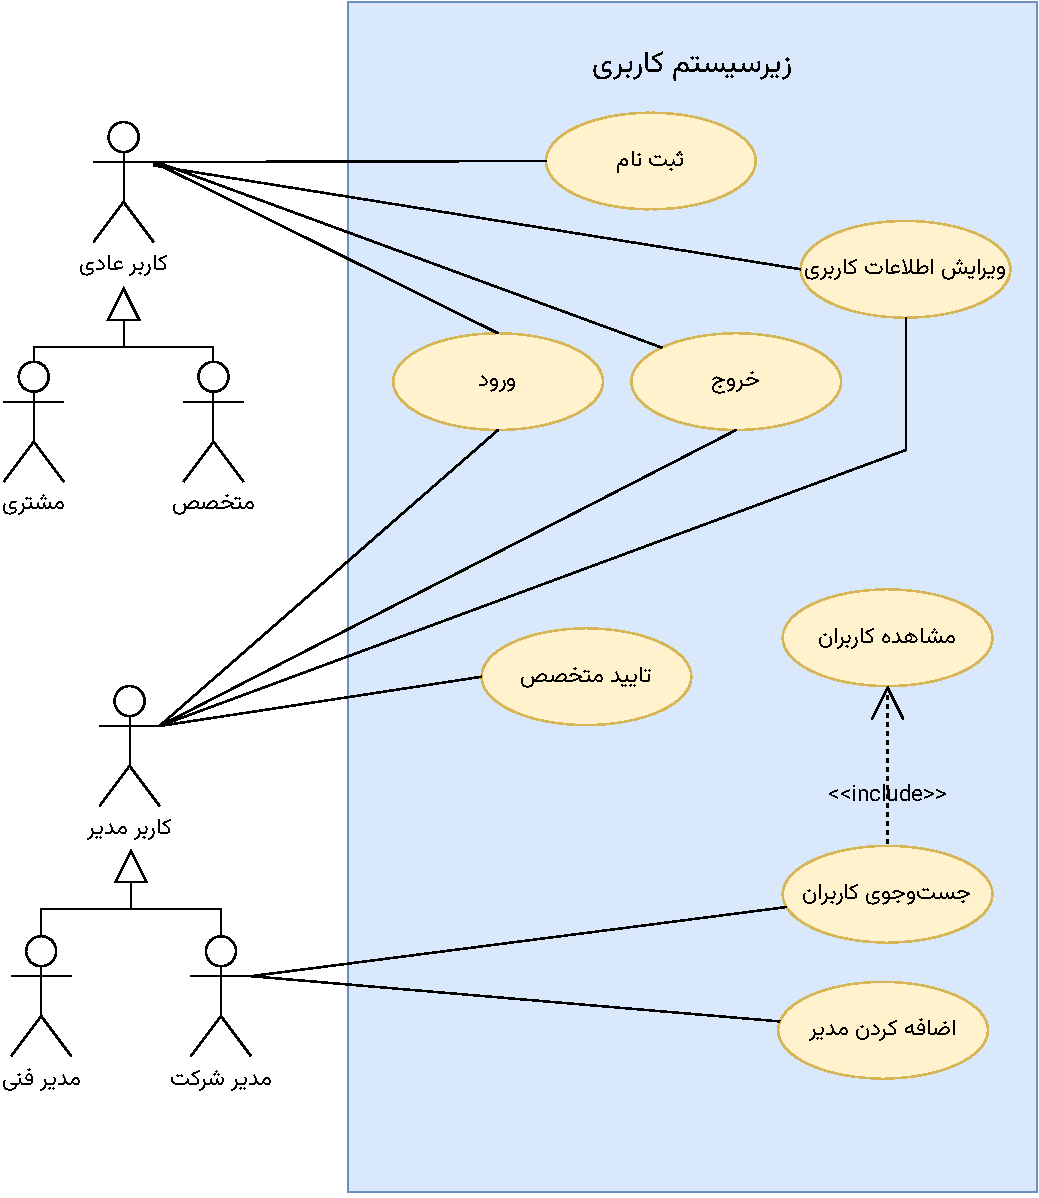
\includegraphics[scale=0.8, page=1]{figs/usecase.pdf}
\caption{زیرسیستم کاربری}
\end{figure}

\FloatBarrier
\newpage


\begin{figure}
\centering
	\includegraphics[scale=0.8, page=2]{figs/usecase.pdf}
\caption{زیرسیستم خدمت‌دهی}
\end{figure}
\FloatBarrier
\newpage

\begin{figure}
\centering
	\includegraphics[scale=0.9, page=3]{figs/usecase.pdf}
\caption{زیرسیستم بازخورد}
\end{figure}
\FloatBarrier
\newpage

\begin{figure}
\centering
	\includegraphics[scale=0.9, page=4]{figs/usecase.pdf}
\caption{زیرسیستم گزارش‌گیری}
\end{figure}
\FloatBarrier
\newpage

\begin{figure}
	\centering
	\includegraphics[scale=0.9, page=5]{figs/usecase.pdf}
	\caption{زیرسیستم مدیریت}
\end{figure}
\FloatBarrier
\newpage

\newpage
\section{فهرست موارد کاربرد}


\subsection{زیرسیستم کاربری}
\renewcommand{\labelenumiii}{\arabic{enumi}.\arabic{enumii}.\arabic{enumiii}}

% ثبث نام
{
\usecase
{ثبت نام}
{۱}
{مشتری یا متخصص، در سایت ثبت نام می‌کنند تا بتوانند از امکانات سایت استفاده کنند.}
{مشتری، متخصص}
{}{کاربر (مشتری یا متخصص) وارد حساب کاربری خود نشده باشد (لاگین نکرده باشد).}
{
\vspace*{-0.6cm}
\begin{enumerate}
	\item 
	کاربر اقدام به ثبت نام در سایت به عنوان متخصص یا مشتری می‌کند.
	\item
	\textbf{تا زمانی که} اطلاعات کاربر به طور کامل وارد نشده است:
	
	\begin{enumerate}[label=\theenumi.\arabic*.]
	\item
	کاربر اطلاعات هویتی شامل نام و نام‌خانوادگی و همچنین شماره تلفن همراه و ایمیل را وارد می‌کند.
	\item 
	کاربر رمز عبور خود را وارد می‌کند.
	
	\item 
	\textbf{اگر} کاربر قصد ثبت نام به عنوان متخصص را داشت:
	\begin{enumerate}
		\item 
		کاربر تخصص‌هایی که در آن‌ها مهارت دارد را وارد می‌کند.
			\item 
		کاربر مدارک تخصصی خود را در صورت وجود ارائه می‌دهد.
		\item 
		کاربر زمان‌های در دسترس برای ارائه‌ی خدمت را وارد می‌کند.
	\end{enumerate}

	\item 
	کاربر اطلاعات خود را ثبت می‌کند.
	
	\item 
	سیستم صحت کلی اطلاعات کاربر را کنترل می‌کند.
	\end{enumerate}
	
	\item 
	سیستم ثبت‌نام موفق را به اطلاع کاربر می‌رساند.
	
	
\end{enumerate}
}
{یک اکانت برای کاربر ساخته می‌شود. در صورتی که کاربر به عنوان متخصص ثبت‌نام کرده باشد، در وضعیت در انتظار تایید توسط مدیر قرار می‌گیرد.}
{\begin{itemize}
		\vspace*{-0.6cm}
		\item انصراف: 
		\item معتبر نبودن ایمیل در مرحله ۲.۱.
		
		
\end{itemize}}
{مورد کاربرد: ثبت نام}


\alternativeflow
% name
{
	ثبت نام:انصراف
}
% id
{1.2}
% brief description
{
	کاربر از ثبت نام منصرف می‌شود.
}
% primary actos
{
	همه کاربران
}
% secondary actors
{}
% preconditons
{
	\begin{itemize}
		\vspace*{-0.6cm}
		\item 
		کاربر در سیستم لاگین نکرده باشد.
		\item
		کاربر از ثبت نام  منصرف شده باشد.
	\end{itemize}
}
% main flow
{
	\vspace*{-0.6cm}
	\begin{enumerate}
		\item 
		روند جایگزین می‌تواند هر موقع آغاز شود.
		\item
		کاربر از ثبت نام  انصراف می‌دهد.
	\end{enumerate}
}
% postconditions
{
	کاربر در سایت ثبت نام نمی‌کند.
}
% table name
{
	روند جایگزین: ثبت نام:انصراف
}

\alternativeflow
% name
{
	ثبت‌ نام:معتبر نبودن ایمیل
}
% id
{۱.۱}
% brief description
{
	اگر کاربر در حین ثبت‌نام ایمیل نامعتبر وارد کرده باشد، پیام خطا می‌گیرد.
}
% primary actos
{
	مشتری یا متخصص
}
% secondary actors
{}
% preconditons
{
	\begin{itemize}
	
		\item
		کاربر ایمیل نامعتبر وارد کرده باشد..
	\end{itemize}
}
% main flow
{
	\vspace*{-0.6cm}
	\begin{enumerate}
		\item 
		روند جایگزین در مرحله ۲.۱ روند اصلی اتفاق می‌افتد.
		\item
		کاربر ایمیل نامعتبری وارد می‌کند.
		\item 
		سیستم خطای ایمیل نامعتبر را نمایش می‌دهد.
	\end{enumerate}
}
% postconditions
{
	نمایش خطای ایمیل نامعتبر به کاربر
}
% table name
{
	روند جایگزین: 	ثبت‌ نام:معتبر نبودن ایمیل
}
}

% ورود
{
\usecase
{ورود}
{۲}
{کاربرانی که در سایت ثبت‌ نام کرده‌اند یا از ابتدا اکانت دارند (شامل مدیر، مشتری و متخصص) وارد حساب کاربری خود می‌شوند.}
{همه کاربران (مدیر، مشتری و متخصص)}
{}
{
		\begin{itemize}
		\item
		کاربر در سیستم لاگین نکرده باشد.
		\item
		اکانتی برای کاربر در سایت وجود داشته باشد.
	\end{itemize}
	
}
{
\begin{enumerate}
	\item 
	کاربر درخواست وارد شدن به حساب کاربری خود را می‌کند.
	
	
	\item 
	کاربر ایمیل و پسورد خود را وارد می‌کند.
	
	\item
	سیستم درستی اطلاعات وارد شده را بررسی می‌کند.
	
	\item
	کاربر احراز هویت شده و وارد حساب کاربری خود می‌شود.
\end{enumerate}
}
{اگر اطلاعات وارد شده درست باشد، کاربر وارد حساب کاربری خود می‌شود.}
{	
	
	\begin{itemize}
	\item
	 انصراف
	
	\item
	اشتباه بودن اطلاعات وارد شده
	\end{itemize}
}
{مورد کاربرد: ورود }

\alternativeflow
% name
{
	ورود:انصراف
}
% id
{1.2}
% brief description
{
	کاربر از ورود منصرف می‌شود.
}
% primary actos
{
	همه کاربران (مدیر، مشتری و متخصص)
}
% secondary actors
{}
% preconditons
{
	\begin{itemize}
		\vspace*{-0.6cm}
		\item 
		کاربر در سیستم لاگین نکرده باشد.
		\item
		کاربر از ورود  منصرف شده باشد.
	\end{itemize}
}
% main flow
{
	\vspace*{-0.6cm}
	\begin{enumerate}
		\item 
		روند جایگزین می‌تواند هر موقع آغاز شود.
		\item
		کاربر از ورود  انصراف می‌دهد.
	\end{enumerate}
}
% postconditions
{
	کاربر وارد سایت نمی‌شود و فرآیند ورود لغو می‌شود.
}
% table name
{
	روند جایگزین: ورود:انصراف
}

\alternativeflow
% name
{
	ورود:اشتباه بودن اطلاعات وارد شده
}
% id
{2.2}
% brief description
{
	اگر کاربر در حین ورود اطلاعات اشتباه وارد کند، پیام خطا گرفته و به ابتدای فرآیند ورود باز می گردد
}
% primary actos
{
	مشتری یا متخصص
}
% secondary actors
{}
% preconditons
{
	\begin{itemize}
		
		\item
		اطلاعات ورودی کاربر نادرست باشد.
	\end{itemize}
}
% main flow
{
	\vspace*{-0.6cm}
	\begin{enumerate}
		\item 
		روند جایگزین در مرحله ۳ روند اصلی اتفاق می‌افتد.
		\item
		کاربر اطلاعات ورود نادرستی وارد می‌کند.
		\item 
		سیستم خطای اطلاعات نامعتبر را نمایش می‌دهد.
		\item
		کاربر به مرحله ۲ روند اصلی باز می‌گردد.
	\end{enumerate}
}
% postconditions
{
	بازگشت کاربر به مرحله ۲ از روند اصلی
}
% table name
{
	روند جایگزین: ورود:اشتباه بودن اطلاعات وارد شده
}
}

% خروج
{
\usecase
{خروج}
{3}
{کاربرانی که در سایت وارد شده‌اند، از حساب کاربری خود خارج می‌شوند}
{همه کاربران (مدیر، مشتری و متخصص)}
{}
{
	\begin{itemize}
		\item
		کاربر در سیستم لاگین کرده باشد.

	\end{itemize}
	
}
{
	\begin{enumerate}
		\item 
		کاربر درخواست خروج از  حساب کاربری خود را می‌کند.
		
		
		\item 
		سیستم کاربر را از حساب کاربری خود خارج می‌کند.
		
		\item
		کاربر به صفحه ورود به سیستم بازگردانده می‌شود.
		
	
	\end{enumerate}
}{کاربر از حساب کاربری خود خارج می‌شود.}
{	
}
{مورد کاربرد: خروج }
}

% جست‌وجوی کاربران
{
\usecase
{جست‌وجوی کاربران}
{۳}
{مدیر شرکت با وارد کردن فیلترهای مختلف به جست‌و‌جوی کاربران می‌پردازد}
{مدیر شرکت}
{}
{
	\begin{itemize}
	\item
	مدیر در سیستم لاگین کرده باشد.
	
	\end{itemize}
 }
{
\begin{enumerate}
	\item 
	مدیر وارد قسمت جست‌وجوی کاربران می‌شود.
	
	\item 
	مدیر اطلاعات لازم برای فیلتر‌های جست‌وجو - شامل نام،‌ نام‌خانوادگی، نوع کاربر (متخصص یا مشتری)، تخصص‌ها در صورت انتخاب نوع متخصص، ایمیل و شماره تلفن- را وارد می‌کند.
	
	\item
	سیستم براساس فیلتر‌های وارد شده در لیست کاربران جست‌وجو می‌کند.
	
	\item 
	کاربرانی که با فیلتر‌های وارد شده تطابق داشته باشند، به عنوان خروجی داده می‌شوند.
	
	\item
	شامل (\lr{Include}) مورد کاربری «مشاهده کاربران»
\end{enumerate}
}
{}
{
\begin{itemize}
	\item	
	انصراف
	
	\item 
	ورود اطلاعات نامعتبر
\end{itemize}
}
{مورد کاربرد: جست‌وجوی کاربران}


\cancelAlternativeFlow{جست‌وجوی کاربران}{مدیر}{1}{فرآیند جست‌وجوی کاربران لغو می‌شود.}


\alternativeflow
% name
{
	جست‌وجوی کاربران:ورود اطلاعات نامعتبر
}
% id
{1.3}
% brief description
{
	هیچ کاربری با اطلاعات وارد شده یافت نمی‌شود.
}
% primary actos
{
	مدیر شرکت
}
% secondary actors
{}
% preconditons
{
	\begin{itemize}
		
		\item
		هیچ کاربری با اطلاعات وارد شده وجود نداشته باشد.
	\end{itemize}
}
% main flow
{
	\vspace*{-0.6cm}
	\begin{enumerate}
		\item 
		روند جایگزین در مرحله ۳ روند اصلی اتفاق می‌افتد.
		\item
		هیچ کاربری با اطلاعات وارد شده یافت نمی‌شود.
		\item 
		سیستم خطای یافت نشدن کاربری با اطلاعات وارد شده را نمایش می‌دهد.
		\item
	\end{enumerate}
}
% postconditions
{
	پیام خطای اطلاعات نامعتبر و یافت نشدن کاربری با این اطلاعات نمایش داده می‌شود.
}
% table name
{
	روند جایگزین: جست‌وجوی کاربران:ورود اطلاعات نامعتبر
}
}

% مشاهده کاربران
{
\usecase
{مشاهده کاربران}
{۴}
{مدیر شرکت اطلاعات کاربرانی که مشخص کرده است را مشاهده می‌کند.}
{مدیر شرکت}
{}
{
		\begin{itemize}
		\item
		مدیر در سیستم لاگین کرده باشد.
		
		\item
		‌کاربرانی که قرار است نمایش داده شوند مشخص شده باشند.
	\end{itemize}
}
{
\begin{enumerate}
	\item 
	سیستم لیست (آی‌دی) کاربرانی که قرار است نمایش داده شوند را از «مورد کاربرد جست‌وجوی کاربران» دریافت می‌کند.
	
	\item
	سیستم کاربران مشخص شده را به همراه تمامی صفات آنان به مدیر نمایش می‌دهد.
\end{enumerate}
}
{
}
{
	\begin{itemize}
		\item 
		وجود نداشتن آی‌دی‌ها
	\end{itemize}
}
{مورد کاربرد: مشاهده کاربران}

\alternativeflow
% name
{
	مشاهده کاربران:وجود‌ نداشتن آی‌دی‌ها
}
% id
{1.3}
% brief description
{
	اگر هیچ کاربری با آی‌دی‌های ذکر شده وجود نداشته باشد، اطلاعات آن نمایش داده نمی‌شود.
}
% primary actos
{
	مدیر شرکت
}
% secondary actors
{}
% preconditons
{
	\begin{itemize}
		
		\item
		هیچ کاربری با اطلاعات وارد شده وجود نداشته باشد.
	\end{itemize}
}
% main flow
{
	\vspace*{-0.6cm}
	\begin{enumerate}
		\item 
		روند جایگزین در مرحله ۲ روند اصلی اتفاق می‌افتد.
		\item
		هیچ کاربری با آی‌دی‌ وارد شده یافت نمی‌شود.
		\item 
		برای این آی‌دی‌ها، اطلاعاتی نمایش داده نشده و نادیده گرفته می‌شوند.
	\end{enumerate}
}
% postconditions
{
	کاربرانی که یافت نشده‌اند، نادیده گرفته شده و اطلاعاتی برای آن‌ها نمایش داده نمی‌شود.
}
% table name
{
	روند جایگزین:  مشاهده کاربران:وجود نداشتن آی‌دی‌ها
}
}


% تایید متخصص
{
\usecase
{تایید متخصص}
{۵}
{کاربر مدیر متخصصی که ثبت نام کرده است را تایید یا رد می‌کند.}
{کاربر مدیر}
{}
{
	\begin{itemize}
	\item 
متخصص در سیستم ثبت‌نام کرده باشد و هنوز تایید نشده باشد.
	
	\item
کاربر مدیر در سیستم لاگین کرده باشد.
\end{itemize}
}
{
\begin{enumerate}
	\item 
	شامل (\lr{Include}) مورد کاربری «جست‌وجوی کاربران»
	\item
	سیستم لیست متخصصانی که تایید نشده‌اند را نمایش می‌دهد.
	
	\item 
کاربر مدیر متخصصی که قصد تایید یا رد آن را دارد انتخاب می‌کند.
	
	\item 
کاربر مدیر بسته به اطلاعات متخصص، رد یا تایید متخصص را مشخص می‌کند.
\item 
وضعیت تایید یا رد شدن متخصص در سیستم ثبت می‌شود.
\end{enumerate}
}
{\begin{itemize}
	\item
	وضعیت متخصص بسته به انتخاب کاربر مدیر، به حالت رد شده یا تایید شده در می‌آید.
\end{itemize}}
{
\begin{itemize}
	\item
	 انصراف
\end{itemize}
}
{مورد کاربرد: تایید متخصص}



\cancelAlternativeFlow{تایید متخصص}{کاربر مدیر}{1}{فرآیند ‌تایید متخصص لغو می‌شود.}

}

% اضافه کردن مدیر جدید
{
\usecase
{اضافه کردن مدیر جدید}
{۶}
{یک مدیر شرکت می‌تواند حساب کاربری برای مدیر جدیدی در شرکت ایجاد کند.}
{مدیر شرکت}
{}
{
	\begin{itemize}
		\item
		مدیر شرکت در سیستم لاگین کرده باشد.
		
	\end{itemize}
}
{
\begin{enumerate}
	\item 
	مدیر شرکت وارد قسمت اضافه کردن مدیر جدید می‌شود.
	
\item
\textbf{تا زمانی که} اطلاعات کاربر به طور کامل وارد نشده است:

\begin{enumerate}[label=\theenumi.\arabic*.]
	\item
	کاربر اطلاعات هویتی شامل نام و نام‌خانوادگی و همچنین شماره تلفن همراه و ایمیل و پسورد را وارد می‌کند.

	
	\item 
	سیستم صحت کلی اطلاعات مدیر شرکت جدید را کنترل می‌کند.
\end{enumerate}

	\item 
سیستم ثبت‌نام موفق را به اطلاع مدیر شرکتی که مراحل اضافه کردن را انجام داده می‌رساند.

\end{enumerate}
}
{
حساب کاربری برای مدیر شرکت جدید ایجاد می‌شود.
}
{\begin{itemize}
		\vspace*{-0.6cm}
		\item انصراف: در صورت انصراف، ایجاد مدیر جدید لغو می‌شود
		\item معتبر نبودن ایمیل در مرحله ۲.۱.
		
		
\end{itemize}}
{مورد کاربرد: اضافه کردن مدیر جدید}

\cancelAlternativeFlow{اضافه کردن مدیر جدید}{مدیر شرکت}{1}{فرآیند اضافه کردن مدیر جدید لغو می‌شود.}


\alternativeflow
% name
{
	اضافه کردن مدیر جدید:معتبر نبودن ایمیل
}
% id
{1.6}
% brief description
{
	اگر مدیر شرکت در حین ثبت‌ایجاد مدیر شرکت جدید ایمیل نامعتبر وارد کرده باشد، پیام خطا می‌گیرد.
}
% primary actos
{
	مدیر شرکت
}
% secondary actors
{}
% preconditons
{
	\begin{itemize}
		
		\item
		مدیر شرکت ایمیل نامعتبر وارد کرده باشد.
	\end{itemize}
}
% main flow
{
	\vspace*{-0.6cm}
	\begin{enumerate}
		\item 
		روند جایگزین در مرحله ۲.۱ روند اصلی اتفاق می‌افتد.
		\item
		مدیر شرکت ایمیل نامعتبری وارد می‌کند.
		\item 
		سیستم خطای ایمیل نامعتبر را نمایش می‌دهد.
	\end{enumerate}
}
% postconditions
{
	نمایش خطای ایمیل نامعتبر به مدیر شرکت
}
% table name
{
	روند جایگزین: 	اضافه کردن مدیر جدید:معتبر نبودن ایمیل
}
}


% ویرایش اطلاعات کاربری
{
	\usecase
	{ویرایش اطلاعات کاربری}
	{9}
	{کاربر اطلاعات کاربری خود را ویرایش می‌کند}
	{همه کاربران}
	{}
	{
		\begin{itemize}
			\item 
		کاربر در سیستم لاگین کرده باشد.
			
		\end{itemize}
	}
	{
		\begin{enumerate}
			\item 
	کاربر وارد قسمت ویرایش اطلاعات کاربری می‌شود.
	
	\textbf{تا زمانی که} اطلاعات جدید کاربر صحیح نیست :
	
	\begin{enumerate}[label=\theenumi.\arabic*.]
			\item
	کاربر اطلاعات کاربری خود شامل نام و نام‌خانوادگی، شماره موبایل و پسورد را عوض می‌کند. (امکان تغییر ایمیل وجود ندارد)
			
			\item
			\textbf{اگر} کاربر متخصص باشد:
			\begin{enumerate}
				\item 
				متخصص در صورت تمایل تخصص‌های خود را تغییر می‌دهد.
				
								\item 
				متخصص در صورت تمایل وضعیت فعال/غیر فعال بودن خود را تغییر می‌دهد.
			\end{enumerate}
			
			\end{enumerate}
		
			\item
			کاربر اطلاعات جدید خود را ثبت می‌کند.
			
			\item
			سیستم ثبت اطلاعات جدید را به کاربر اطلاع می‌دهد.
			
		\end{enumerate}
	}
	{\begin{itemize}
			\item
			اطلاعات جدید کاربر در سیستم ثبت می‌شود.
	\end{itemize}}
	{
		\begin{itemize}
			\item انصراف
		\end{itemize}
	}
	{مورد کاربرد: ویرایش اطلاعات کاربری}
	
	
	\cancelAlternativeFlow{ویرایش اطلاعات کاربری}{کاربر}{1}{ویرایش اطلاعات کاربر لغو می‌شود.}
	
}


\newpage
\subsection{زیرسیستم خدمت‌دهی}

% فیلتر و مرتب‌سازی درخواست‌ها
{
\usecase
% name
{فیلتر و مرتب‌سازی درخواست‌ها}
% id
{8}
% brief description
{متخصص می‌تواند در خواست‌های مرتبط با خودش را براساس معیارهای مختلف (شامل اطلاعات مشتری درخواست دهنده، تخصص‌ خواسته شده و زمان) اولویت بندی و فیلتر کند.}
% primary actos
{متخصص}
% secondary actors
{}
% preconditons
{	
	\begin{itemize}
		\vspace*{-0.6cm}
		\item 
		متخصص در سیستم لاگین کرده باشد.
	\end{itemize}
}
% main flow
{
	\vspace*{-0.6cm}
	\begin{enumerate}
		\item 
		متخصص وارد قسمت درخواست‌ها می‌شود.
		\item
		متخصص فیلترهای لازم را اعمال کرده و معیار مرتب‌سازی را انتخاب می‌کند.
		\item
		سیستم درخواست‌هایی که با فیلترها مطابقت دارند را لیست می‌کند.
		
		\item
		\textbf{به ازای هر} هر درخواست:
		
		\begin{enumerate}[label=\theenumi.\arabic*.]
			\item
			شامل (Include) مورد کاربری «مشاهده جزئیات درخواست»
		\end{enumerate}
	
	\end{enumerate}
}
% postconditions
{}
% alternative flows
{
	\begin{itemize}
		\item
		انصراف
\end{itemize}
}
% table name
{
	مورد کاربرد: فیلتر و مرتب‌سازی درخواست‌ها
}

\cancelAlternativeFlow{فیلتر و مرتب‌سازی درخواست‌ها}{متخصص}{1}{فرآیند فیلتر و مرتب‌سازی درخواست‌ها لغو می‌شود.}
}


% مشاهده درخواست‌ها
{
\usecase
% name
{مشاهده درخواست‌ها}
% id
{8}
% brief description
{مشتری خدماتی که تاکنون درخواست کرده است به همراه وضعیت آن‌ها را مشاهده می‌کند.}
% primary actos
{مشتری}
% secondary actors
{}
% preconditons
{	
	\begin{itemize}
		\vspace*{-0.6cm}
		\item 
		مشتری در سیستم لاگین کرده باشد.
	\end{itemize}
}
% main flow
{
	\vspace*{-0.6cm}
	\begin{enumerate}
		\item
		مشتری درخواست دیدن درخواست‌هایی که تاکنون ثبت کرده است را می‌دهد.
		\item
		سیستم درخواست‌هایی که توسط مشتری ثبت شده است را به صورت مرتب شده به همراه وضعیت آن (انجام شده، در انتظار پذیرش توسط متخصص، در انتظار تعیین متخصص، لغو شده، در حال انجام) نمایش می‌دهد.
		
		\item
		\textbf{به ازای هر} هر درخواست:
		
		\begin{enumerate}[label=\theenumi.\arabic*.]
			\item
			شامل (Include) مورد کاربری «مشاهده جزئیات درخواست»
		\end{enumerate}
	\end{enumerate}
}
% postconditions
{}
% alternative flows
{
	\begin{itemize}
		\item
		انصراف
	\end{itemize}
}
% table name
{
	مورد کاربرد: فیلتر و مرتب‌سازی درخواست‌ها
}

\cancelAlternativeFlow{مشاهده درخواست‌ها}{مشتری}{1}{فرآیند مشاهده درخواست‌ها لغو می‌شود.}
}

% مشاهده جزئیات درخواست

{
	\usecase
	{مشاهده جزئیات درخواست}
	{۴}
	{کاربر اطلاعات خدمتی که مشخص کرده است را مشاهده می‌کند.}
	{کاربر}
	{}
	{
		\begin{itemize}
			\item
			کاربر در سیستم لاگین کرده باشد.
			
			\item
			‌خدمتی که قرار است نمایش داده شود مشخص شده باشند.
		\end{itemize}
	}
	{
		\begin{enumerate}
			\item 
			سیستم آی‌دی خدمتی که قرار است نمایش داده شوند را از «مورد کاربرد  فیلتر و مرتب‌سازی درخواست‌ها»  یا «مشاهده درخواست‌ها» دریافت می‌کند.
			
			\item
			سیستم خدمت مشخص شده را به همراه تمامی صفات آن به کاربر نمایش می‌دهد.
		\end{enumerate}
	}
	{
	}
	{
		\begin{itemize}
			\item 
			وجود نداشتن آی‌دی‌
		\end{itemize}
	}
	{مورد کاربرد: مشاهده جزئیات درخواست}
	
	\alternativeflow
	% name
	{
		مشاهده جزئیات درخواست:وجود‌ نداشتن آی‌دی‌
	}
	% id
	{1.3}
	% brief description
	{
		اگر هیچ خدمتی با آی‌دی‌ ذکر شده وجود نداشته باشد، اطلاعات آن نمایش داده نمی‌شود.
	}
	% primary actos
	{
		کاربر عادی
	}
	% secondary actors
	{}
	% preconditons
	{
		\begin{itemize}
			
			\item
			هیچ خدمتی با اطلاعات وارد شده وجود نداشته باشد.
		\end{itemize}
	}
	% main flow
	{
		\vspace*{-0.6cm}
		\begin{enumerate}
			\item 
			روند جایگزین در مرحله ۲ روند اصلی اتفاق می‌افتد.
			\item
			هیچ خدمتی با آی‌دی‌ وارد شده یافت نمی‌شود.
			\item 
			برای این آی‌دی‌ها، اطلاعاتی نمایش داده نشده و نادیده گرفته می‌شوند.
		\end{enumerate}
	}
	% postconditions
	{
		خدمتی که یافت نشده‌، نادیده گرفته شده و اطلاعاتی برای آن نمایش داده نمی‌شود.
	}
	% table name
	{
		روند جایگزین: مشاهده جزئیات درخواست:وجود‌ نداشتن آی‌دی‌
	}
}


% انتخاب متخصص برای خدمت
{
\usecase
% name
{انتخاب متخصص برای خدمت}
% id
{8}
% brief description
{مشتری برای خدمت درخواستی خود، متخصصی را انتخاب می‌کند تا در صورت پذیرش متخصص، آن متخصص کار را انجام بدهد.}
% primary actos
{مشتری}
% secondary actors
{}
% preconditons
{	
	\begin{itemize}
		\vspace*{-0.6cm}
		\item 
		مشتری در سیستم لاگین کرده باشد.
		\item
		حداقل یک درخواست به اتمام نرسیده و ثبت شده از سوی مشتری وجود داشته باشد.
	\end{itemize}
}
% main flow
{
	\vspace*{-0.6cm}
	\begin{enumerate}
		\item 
		شامل (Include) مشاهده درخواست‌ها
			\item 
مشتری یک درخواست انجام نشده انتخاب می‌کند.
	\item
	شامل ({Include}) مورد کاربری «جست‌وجو و مشاهده متخصصین»
	\item
	 مشتری برای درخواست انجام نشده‌اش، یک متخصص را انتخاب می‌کند.
	\item
	سیستم درخواست مشتری را به متخصص اعلام می‌کند.
	\end{enumerate}
}
% postconditions
{
درخواست مشتری برای خدمات به متخصص مشخص شده ارسال می‌شود.
}
% alternative flows
{
	\begin{itemize}
		\item
		انصراف
	\end{itemize}
}
% table name
{
	مورد کاربرد: انتخاب متخصص برای خدمت
}

\cancelAlternativeFlow{انتخاب متخصص برای خدمت}{مشتری}{1}{فرآیند انتخاب متخصص برای خدمت لغو می‌شود.}
}



% پذیرش درخواست مستقیم مشتری
{
	\usecase
	% name
	{پذیرش درخواست مستقیم مشتری}
	% id
	{9}
	% brief description
	{متخصص می‌تواند در صورت درخواست مستقیم مشتری برای ارائه خدمت، آن را بپذیرد}
	% primary actos
	{متخصص}
	% secondary actors
	{}
	% preconditons
	{	
		\begin{itemize}
			\vspace*{-0.6cm}
			\item 
			متخصص در سیستم لاگین کرده باشد.
			\item
			مشتری درخواست خدمت را در سیستم ثبت کرده باشد.
			\item
			مشتری درخواست خدمت‌دهی از متخصص خاص را ارسال کرده باشد.
		\end{itemize}
	}
	% main flow
	{ 
		\vspace*{-0.6cm}
		\begin{enumerate}
			\item
			متخصص پیام درخواست کاربر از او برای خدمت‌دهی را مشاهده می‌کند.
			\item 
			شامل (Include) مورد کاربری «مشاهده جزئیات درخواست»
			\item
			پس از مشاهده‌ی جزییات، متخصص برای انجام این درخواست اعلام آمادگی می‌کند.
				\item
		سیستم وضعیت درخواست را بروزرسانی می‌کند.
			\item
			سیستم اعلام آمادگی متخصص را به مشتری اطلاع می‌دهد و موفقیت آمیز بودن آن را به متخصص اعلام می‌کند.
		\end{enumerate}
	}
	% postconditions
	{درخواست پذیرش متخصص به مشتری ارسال می‌شود.}
	% alternative flows
	{
		\begin{itemize}
			\vspace*{-0.6cm}
			\item
			رد خدمت
			\item 
			 عدم امکان پذیرش
		\end{itemize}
	}
	% table name
	{
		مورد کاربرد: پذیرش درخواست مستقیم مشتری
	}
	
	\alternativeflow
	% name
	{
		پذیرش درخواست مستقیم مشتری:رد درخواست
	}
	% id
	{1.9}
	% brief description
	{
		متخصص می‌تواند درخواست‌ مستقیم مشتری برای خدمت‌دهی در یک مورد خاص را رد کند.
	}
	% primary actos
	{
		متخصص
	}
	% secondary actors
	{}
	% preconditons
	{
		\begin{itemize}
			\vspace*{-0.6cm}
			\item 
			متخصص در سیستم لاگین کرده باشد.
			\item
			متخصص در حال مشاهده‌ی یک درخواست باشد.
		\end{itemize}
	}
	% main flow
	{
		\vspace*{-0.6cm}
		\begin{enumerate}
			\item 
			روند جایگزین در مرحله‌ی ۳ می‌تواند آغاز شود.
			\item
			متخصص رد درخواست را تایید می‌کند.
							\item
		سیستم وضعیت درخواست را بروزرسانی می‌کند.
				\item
سیستم رد درخواست را به مشتری اطلاع می‌دهد.
		
		\end{enumerate}
	}
	% postconditions
	{
		رد درخواست به اطلاع مشتری می‌رسد.
	}
	% table name
	{
		روند جایگزین:پذیرش درخواست مستقیم مشتری: رد درخواست
	}

	\alternativeflow
	% name
	{
		پذیرش درخواست مستقیم مشتری:  عدم امکان پذیرش
	}
	% id
	{1.9}
	% brief description
	{
 متخصص به علت رسیدن به حد مجاز پذیرش درخواست نمی‌تواند درخواست مشتری را بپذیرد.
	}
	% primary actos
	{
		متخصص
	}
	% secondary actors
	{}
	% preconditons
	{
		\begin{itemize}
			\vspace*{-0.6cm}
			\item 
			متخصص در سیستم لاگین کرده باشد.
			\item
			متخصص در حال مشاهده‌ی یک درخواست باشد.
		\end{itemize}
	}
	% main flow
	{
		\vspace*{-0.6cm}
		\begin{enumerate}
			\item 
			روند جایگزین بعد از مرحله‌ی ۳ آغاز می‌شود.
			\item
			سیستم به متخصص اعلام می‌کند به علت رسیدن به حد مجاز درخواست‌های پذیرفته شده‌ی به اتمام نرسیده، نمی‌تواند درخواست را قبول کند.
			
		\end{enumerate}
	}
	% postconditions
	{
		درخواست پذیرفته نمی‌شود و در حالت انتظار باقی می‌ماند.

	}
	% table name
	{
		روند جایگزین:پذیرش درخواست مستقیم مشتری: عدم امکان پذیرش
	}
}


% پذیرش خدمت
{
\usecase
% name
{پذیرش درخواست دلخواه}
% id
{9}
% brief description
{متخصص می‌تواند برای انجام خدمت مرتبط با حوزه‌ی تخصص خودش داوطلب شود.}
% primary actos
{متخصص}
% secondary actors
{}
% preconditons
{	
	\begin{itemize}
		\vspace*{-0.6cm}
		\item 
		متخصص در سیستم لاگین کرده باشد.
		\item
		مشتری درخواست خدمت را در سیستم ثبت کرده باشد.
	\end{itemize}
}
% main flow
{
	\vspace*{-0.6cm}
	\begin{enumerate}
		\item 
		شامل (Include) مورد کاربری «فیلتر و مرتب‌سازی درخواست‌ها»
		\item
		متخصص یک درخواست را انتخاب می‌کند تا جزییات آن نمایش داده شود.
				\item
			شامل (Include) مورد کاربری «مشاهده جزئیات درخواست»
		\item 
		\textbf{اگر} تعداد کل درخواست‌های متخصص در ماه کمتر از حد مجاز براساس امتیاز وی بود:
		\begin{enumerate}[label=\theenumi.\arabic*.]
			\item 
		
		\item
		پس از مشاهده‌ی جزییات، متخصص برای انجام این درخواست اعلام آمادگی می‌کند.
		\item
		سیستم اعلام آمادگی متخصص را به مشتری اطلاع می‌دهد و موفقیت آمیز بودن آن را به متخصص اعلام می‌کند.
		\end{enumerate}
	\end{enumerate}
}
% postconditions
{درخواست پذیرش متخصص به مشتری ارسال می‌شود.}
% alternative flows
{
	\begin{itemize}
		\vspace*{-0.6cm}
		\item
		رد خدمت
		\item
		 عدم امکان پذیرش
	\end{itemize}
}
% table name
{
	مورد کاربرد: پذیرش درخواست دلخواه
}

\alternativeflow
% name
{
	 پذیرش درخواست دلخواه:رد خدمت
}
% id
{1.9}
% brief description
{
	متخصص می‌تواند درخواست‌های ارسال شده را رد کند.
}
% primary actos
{
	متخصص
}
% secondary actors
{}
% preconditons
{
	\begin{itemize}
		\vspace*{-0.6cm}
		\item 
		متخصص در سیستم لاگین کرده باشد.
		\item
		متخصص در حال مشاهده‌ی یک درخواست باشد.
	\end{itemize}
}
% main flow
{
	\vspace*{-0.6cm}
	\begin{enumerate}
		\item 
		روند جایگزین در مرحله‌ی مشاهده‌ی جزییات سفارش می‌تواند آغاز شود.
		\item
		متخصص دلیل رد درخواست را وارد می‌کند.
		
		\item
		متخصص رد درخواست را تایید می‌کند.
		\item
		این درخواست دیگر در لیست درخواست‌ها برای متخصص نمایش داده نمی‌شود.
	\end{enumerate}
}
% postconditions
{
	درخواست از دید متخصص پنهان می‌شود.
}
% table name
{
روند جایگزین: پذیرش درخواست دلخواه: رد خدمت
}

\alternativeflow
% name
{
پذیرش درخواست دلخواه:  عدم امکان پذیرش
}
% id
{1.9}
% brief description
{
	متخصص به علت رسیدن به حد مجاز پذیرش درخواست نمی‌تواند درخواست را بپذیرد.
}
% primary actos
{
	متخصص
}
% secondary actors
{}
% preconditons
{
	\begin{itemize}
		\vspace*{-0.6cm}
		\item 
		متخصص در سیستم لاگین کرده باشد.
		\item
		متخصص در حال مشاهده‌ی یک درخواست باشد.
	\end{itemize}
}
% main flow
{
	\vspace*{-0.6cm}
	\begin{enumerate}
		\item 
		روند جایگزین بعد از مرحله‌ی ۳ آغاز می‌شود.
		\item
		سیستم به متخصص اعلام می‌کند به علت رسیدن به حد مجاز درخواست‌های پذیرفته شده‌ی به اتمام نرسیده، نمی‌تواند درخواست را قبول کند.
		
	\end{enumerate}
}
% postconditions
{
	درخواست پذیرفته نمی‌شود و در حالت انتظار باقی می‌ماند.
	
}
% table name
{
	روند جایگزین:پذیرش درخواست دلخواه: عدم امکان پذیرش
}

}

% پذیرش متخصص
{
\usecase
% name
{پذیرش متخصص}
% id
{10}
% brief description
{مشتری می‌تواند متخصص داوطلب شده را تایید کند.}
% primary actos
{مشتری}
% secondary actors
{}
% preconditons
{	
	\begin{itemize}
		\vspace*{-0.6cm}
		\item 
		مشتری در سیستم لاگین کرده باشد.
		\item
		مشتری درخواست خدمت را در سیستم ثبت کرده باشد.
		\item
		یک متخصص برای انجام خدمت داوطلب شده باشد.
	\end{itemize}
}
% main flow
{
	\vspace*{-0.6cm}
	\begin{enumerate}
		\item
					متخصص پیام پذیرش متخصص را مشاهده می‌کند.
		\item
سیستم اطلاعات متخصص را نشان می‌دهد.
		\item 
		در صورت موافقت، مشتری متخصص را تایید می‌کند.
		\item 
		سیستم متخصص را برای انجام خدمت ثبت می‌کند و پیامی برای اطلاع متخصص می‌فرستد.
	\end{enumerate}
}
% postconditions
{متخصص برای انجام خدمت ثبت می‌شود.}
% alternative flows
{
	\begin{itemize}
		\vspace*{-0.6cm}
		\item
		رد متخصص
	\end{itemize}
}
% table name
{
	مورد کاربرد: پذیرش متخصص
}

\alternativeflow
% name
{
	 پذیرش متخصص:رد متخصص
}
% id
{1.10}
% brief description
{
	مشتری می‌تواند متخصص داوطلب شده را رد کند.
}
% primary actos
{
	مشتری
}
% secondary actors
{}
% preconditons
{
	\begin{itemize}
		\vspace*{-0.6cm}
		\item 
		مشتری در سیستم لاگین کرده باشد.
		\item
		مشتری در حال مشاهده‌ی متخصص داوطلب شده باشد.
	\end{itemize}
}
% main flow
{
	\vspace*{-0.6cm}
	\begin{enumerate}
		\item 
		روند جایگزین در مرحله‌ی مشاهده‌ی متخصص داوطلب شده می‌تواند آغاز شود.
		\item
		مشتری دلیل رد متخصص را وارد می‌کند.
		\item
		مشتری رد متخصص را تایید می‌کند.
			\item
			سیستم متخصص را از درخواست حذف می‌کند.
		\item
		سیستم متخصص را از رد شدن مطلع می‌کند.
	\end{enumerate}
}
% postconditions
{
متخصص از درخواست حذف می‌شود و درخواست دوباره در معرض دید متخصصین قرار می‌گیرد.
}
% table name
{
روند جایگزین:پذیرش متخصص:رد متخصص
}
}


% لغو درخواست خدمت
{
\usecase
% name
{
	لغو درخواست خدمت
}
% id
{11}
% brief description
{
	مشتری یا کاربر مدیر می‌تواند خدمت درخواست شده را لغو کند.
}
% primary actos
{
مشتری یا کاربر مدیر
}
% secondary actors
{
	متخصص
}
% preconditons
{
	\begin{itemize}
		\vspace*{-0.6cm}
\item 
مشتری یا کاربر مدیر در سیستم لاگین کرده باشد.
	\end{itemize}
}
% main flow
{
	\vspace*{-0.6cm}
	\begin{enumerate}
\item 
مشتری یا کاربر مدیر درخواست لغو خدمت می‌دهد.
\item اگر درخواست‌کننده مشتری باشد:
سیستم درخواست‌های خدمت تایید نشده مشتری را به وی نشان می‌دهد. 
\item اگر درخواست‌کننده کاربر مدیر باشد:
سیستم تمام درخواست‌های انجام نشده‌ی سیستم را به وی نشان می‌دهد.  
\item
مشتری یا کاربر مدیر خدمتی که قصد لغو آن دارد را انتخاب می‌کند.
\item
			شامل (Include) مورد کاربری «مشاهده جزئیات درخواست»
\item
مشتری یا کاربر مدیر لغو خدمت را تایید می‌کند.
\item
خدمت از لیست خدمت‌های درخواستی حذف می‌شود.
\item
\textbf{اگر} متخصصی درخواست را تایید کرده بود یا آن را انتخاب کرده بود و منتظر تایید شدن آن بود:
\begin{enumerate}[label=\theenumi.\arabic*.]
	\item 
لغو درخواست به متخصص اطلاع داده می‌شود.

\end{enumerate}

	\end{enumerate}
}
% postconditions
{
		\begin{itemize}
		\vspace*{-0.6cm}
		\item 
خدمت بین خدمت‌های درخواستی نشان داده نمی‌شود و متخصصی نمی‌تواند آن را انتخاب کند.
		\item 
متخصصی درخواست را تایید کرده باشد یا آن را انتخاب کرده و منتظر تایید آن توسط مشتری باشد اطلاع پیدا می‌کند.
	\end{itemize}

}
% alternative flows
{
			\begin{itemize}
		\vspace*{-0.6cm}
		\item
انصراف
\end{itemize}
}
% table name
{
	مورد کاربرد: لغو درخواست خدمت
}



\cancelAlternativeFlow{لغو درخواست خدمت}{مشتری یا کاربر مدیر }{1}{}
}





% جست‌وجو و مشاهده متخصصین

{
\usecase
% name
{جست‌وجو و مشاهده متخصصین}
% id
{12}
% brief description
{
	مشتری لیستی از متخصصین یک حوزه‌ی مشخص / در دسترس مشاهده کند.
}
% primary actors
{مشتری}
% secondary actors
{}
% preconditons
{
	مشتری در سیستم لاگین کرده باشد.
}
% main flow
{
	\vspace*{-0.6cm}
	\begin{enumerate}
		\item 
		مورد کاربرد با انتخاب «مشاهده‌ی متخصصین» توسط مشتری آغاز می‌شود.
		\item 
		مشتری شرایط مدنظر خود برای مشاهده‌ی متخصصین (حوزه‌های تخصص و امتیاز) مرتبط را وارد می‌کند.
		\item 
		لیستی از متخصصین مورد جست‌وجو به مشتری نمایش داده می‌شود.
	\end{enumerate}
}
% postconditions
{مشتری لیستی از متخصصین مدنظر خود دریافت می‌کند.}
% alternative flows
{
	\begin{itemize}
		\vspace*{-0.6cm}
		\item انصراف
	\end{itemize}
}
% table name
{
	مورد کاربرد: جست‌وجو و مشاهده متخصصین
}

\cancelAlternativeFlow{جست‌وجو و مشاهده متخصصین}{مشتری}{1}{}
}

%  ثبت درخواست  
{
\usecase
% name
{ثبت درخواست}
% id
{13}
% brief description
{
	مشتری با مشاهده خدمات موجود و متخصصین در دسترس و پر کردن فرم اطلاعات درخواست خدمت، یک درخواست خدمات جدید ثبت می‌کند.
}
% primary actors
{مشتری}
% secondary actors
{}
% preconditons
{
	مشتری در سیستم لاگین کرده باشد.
}
% main flow
{
	\vspace*{-0.6cm}
	\begin{enumerate}
		\item 
		مورد کاربرد با انتخاب «ثبت درخواست جدید» توسط مشتری شروع می‌شود.
		\item 
		Include (جست‌وجو و مشاهده متخصصین)
		\item 
		مشتری فرم درخواست جدید را تکمیل کرده و ارسال می‌کند.
				\item 
		\textbf{تا زمانی که}
		اطلاعات ناقص در فرم وجود دارد یا درخواست انجام نشده‌ای با خدمت مشابه درخواست جدید وجود دارد:
		\begin{enumerate}[label=\theenumi.\arabic*.]
						\item 
سیستم مشکل را به مشتری اطلاع می‌دهد
			\item 
			مشتری اطلاعات فرم را اصلاح می‌کند.
		\end{enumerate}
		\item
مشتری درخواست را تایید می‌کند.
		\item 
		درخواست در سیستم ذخیره می‌شود .
		\item 
		به متخصصین با تخصص مشابه درخواست اطلاع داده می‌شود.
		
	\end{enumerate}
}
% postconditions
{یک درخواست خدمت جدید در سیستم ثبت می‌شود.}
% alternative flows
{
	\begin{itemize}
		\vspace*{-0.6cm}
		\item انصراف
	\end{itemize}
}
% table name
{
	مورد کاربرد: ثبت درخواست
}


\cancelAlternativeFlow{ثبت درخواست}{مشتری}{1}{}
}







%  ثبت زمان انجام شدن خدمت

{
\usecase
% name
{ثبت زمان انجام شدن خدمت}
% id
{18}
% brief description
{متخصص زمان پایان خدمت خود را در سیستم ثبت می‌کند.}
% primary actors
{متخصص}
% secondary actors
{}
% preconditons
{متخصص در سیستم لاگین کرده باشد.}
% main flow
{
	\vspace*{-0.6cm}
	\begin{enumerate}
		\item مورد کاربرد توسط متخصص با دریافت لیست خدماتی که ارائه کرده آغاز می‌شود.
		\item متخصص خدمت مورد نظر خود را از لیست انتخاب می‌کند.
		\item متخصص زمان پایان انجام آن خدمت را در سیستم ثبت می‌کند.
	\end{enumerate}
}
% postconditions
{زمان انجام خدمت در سیستم ثبت می‌شود.}
% alternative flows
{
	\begin{itemize}
		\vspace*{-0.6cm}
		\item انصراف
	\end{itemize}
}
% table name
{
	مورد کاربرد: ثبت زمان انجام شدن خدمت
}

\cancelAlternativeFlow{ثبت زمان انجام شدن خدمت}{متخصص}{1}{}
}


% ویرایش درخواست

{
	\usecase
	% name
	{ویرایش درخواست}
	% id
	{18}
	% brief description
	{مشتری قبل از پذیرفته شدن درخواستش، آن را ویرایش می‌کند.}
	% primary actors
	{مشتری}
	% secondary actors
	{}
	% preconditons
	{
		
		\begin{itemize}
			\item
			مشتری در سیستم لاگین کرده باشد.
			
			\item 
			درخواست در وضعیت پذیرفته نشده باشد.
			
		\end{itemize}	
		
		
	}
	% main flow
	{
		\vspace*{-0.6cm}
		\begin{enumerate}
			\item
				شامل (Include) مشاهده درخواست‌ها
				
				\item
				پس از مشاهده درخواست، درخواست برای ویرایش انتخاب می‌شود.
				
				\item 
				\textbf{تا زمانی که}
				اطلاعات ناقص در فرم وجود دارد:
				\begin{enumerate}[label=\theenumi.\arabic*.]
					\item 
	مشتری درخواست شامل جزئیات آن، زمان انجام و تخصص‌های مورد نیاز را ویرایش می‌کند.
				\end{enumerate}
				\item 
			مشتری درخواست ویرایش شده را ثبت می‌کند.
				
			
		\end{enumerate}
	}
	% postconditions
	{اطلاعات جدید درخواست در سیستم ثبت می‌شود.}
	% alternative flows
	{
		\begin{itemize}
			\vspace*{-0.6cm}
			\item انصراف
		\end{itemize}
	}
	% table name
	{
		مورد کاربرد: ویرایش درخواست
	}
	
	\cancelAlternativeFlow{ویرایش درخواست}{مشتری}{1}{فرآیند ویرایش درخواست لغو می‌شود.}
}

% ====================== مشاهده‌ی خدمات ارائه شده به طور دسته‌بندی شده
% TODO


\newpage

\subsection{زیرسیستم بازخورد}

% ارزیابی خدمت دریافت شده
{
\usecase
% name
{
	ارزیابی خدمت دریافت شده
}
% id
{19}
% brief description
{
	مشتری خدمتی که از متخصص دریافت کرده است را ارزیابی می‌کند و بازخورد می‌دهد.
}
% primary actos
{
	مشتری
}
% secondary actors
{}
% preconditons
{
		\begin{itemize}
		\vspace*{-0.6cm}
		\item 
		مشتری در سیستم لاگین کرده باشد. 
	\end{itemize}
}
% main flow
{
	\vspace*{-0.6cm}
	\begin{enumerate}
		\item 
		مشتری درخواست مشاهده لیست خدمت‌‌هایی که دریافت کرده است را می‌دهد.
		 \item
		 سیستم خدمات دریافت شده‌ی مشتری را نشان می‌دهد.
		\item
		مشتری یکی از خدمت‌هایی که دریافت کرده را انتخاب می‌کند.

		\item
سیستم معیارهای ارزیابی  به مشتری نشان می‌دهد.
		\item 
مشتری به خدمت ارائه شده بین $0.5$ تا $5$ ستاره برای هر معیار می‌دهد.

			\item 
	\textbf{اگر} مشتری تمایل به ارائه‌ی توضیحات داشت:
				\begin{enumerate}[label=\theenumi.\arabic*.]
		\item 
		مشتری توضیحات مدنظر را وارد می‌کند. 
	\end{enumerate}
		\item
		سیستم امتیازها و نظر ثبت شده را ذخیره می‌کند و ذخیره موفق بازخوردها را به اطلاع مشتری می‌رساند.
		
	\end{enumerate}
}
% postconditions
{
امتیازها و نظرات کاربر در سیستم ذخیره می‌شوند.
}
% alternative flows
{
	\begin{itemize}
		\vspace*{-0.6cm}
		\item 
		انصراف
	\end{itemize}
}
% table name
{
	مورد کاربرد: ارزیابی خدمت دریافت شده
}





\alternativeflow
% name
{
ارزیابی خدمت دریافت شده:انصراف
}
% id
{1.19}
% brief description
{
مشتری از ارائه‌ی بازخورد نسبت به خدمت دریافت شده منصرف می‌شود.
}
% primary actos
{
	مشتری
}
% secondary actors
{}
% preconditons
{
	\begin{itemize}
		\vspace*{-0.6cm}
		\item 
		مشتری در سیستم لاگین کرده باشد.
		\item
		مشتری از ارائه‌ی بازخورد منصرف شده باشد.
	\end{itemize}
}
% main flow
{
	\vspace*{-0.6cm}
	\begin{enumerate}
		\item 
		روند جایگزین می‌تواند هر موقع آغاز شود.
		\item
		مشتری از ارائه‌ی بازخورد انصراف می‌دهد.
	\end{enumerate}
}
% postconditions
{
امتیاز و نظر مشتری ذخیره نمی‌شود.
}
% table name
{
روند جایگزین: ارزیابی خدمت دریافت شده:انصراف
}


}

% ارزیابی دریافت خدمت ارائه شده
{
\usecase
% name
{
	ارزیابی دریافت خدمت ارائه شده
}
% id
{20}
% brief description
{
	متخصص نسبت به خدمتی که ارائه کرده و فرد دریافت‌کننده‌ی خدمت بازخورد می‌دهد.
}
% primary actos
{
	متخصص
}
% secondary actors
{}
% preconditons
{
	\begin{itemize}
		\vspace*{-0.6cm}
		\item 
		متخصص در سیستم لاگین کرده باشد.
	\end{itemize}
}
% main flow
{
	\vspace*{-0.6cm}
	\begin{enumerate}
		\item 
		متخصص لیست خدمت‌هایی که ارائه کرده است را مشاهده می‌کند.
		\item
		متخصص یکی از خدمت‌هایی که ارائه کرده را انتخاب می‌کند.

\item
سیستم معیارهای ارزیابی  به متخصص نشان می‌دهد.
\item 
متخصص به خدمت ارائه شده بین $0.5$ تا $5$ ستاره برای هر معیار می‌دهد.

\item 
\textbf{اگر} متخصص تمایل به ارائه‌ی توضیحات داشت:
\begin{enumerate}[label=\theenumi.\arabic*.]
	\item 
	متخصص توضیحات مدنظر را وارد می‌کند. 
\end{enumerate}
\item
سیستم امتیازها و نظر ثبت شده را ذخیره می‌کند و ذخیره موفق بازخوردها را به اطلاع متخصص می‌رساند.

	\end{enumerate}
}
% postconditions
{
	امتیازها و نظرات متخصص در سیستم ذخیره می‌شوند.
}
% alternative flows
{
	\begin{itemize}
		\vspace*{-0.6cm}
		\item 
		انصراف
	\end{itemize}
}
% table name
{
	مورد کاربرد: ارزیابی دریافت خدمت ارائه شده
}




\alternativeflow
% name
{
	ارزیابی دریافت خدمت ارائه شده:انصراف
}
% id
{1.20}
% brief description
{
	متخصص از ارائه‌ی بازخورد نسبت به خدمت ارائه شده منصرف می‌شود.
}
% primary actos
{
	متخصص
}
% secondary actors
{}
% preconditons
{
	\begin{itemize}
		\vspace*{-0.6cm}
		\item 
		متخصص در سیستم لاگین کرده باشد.
		\item
		متخصص از ارائه‌ی بازخورد منصرف شده باشد.
	\end{itemize}
}
% main flow
{
	\vspace*{-0.6cm}
	\begin{enumerate}
		\item 
		روند جایگزین می‌تواند هر موقع آغاز شود.
		\item
		متخصص از ارائه‌ی بازخورد انصراف می‌دهد.
	\end{enumerate}
}
% postconditions
{
	امتیاز و نظرات متخصص ذخیره نمی‌شود.
}
% table name
{
	روند جایگزین: ارزیابی دریافت خدمت ارائه شده:انصراف
}
}



% مشاهده لیست معیارهای ارزیابی
{
\usecase
% name
{
مشاهده لیست معیارهای ارزیابی
}
% id
{
	21
}
% brief description
{
مدیر شرکت می‌تواند معیارهای ارزیابی متخصصیان و مشتریان سیستم را مشاهده کند.
}
% primary actos
{
مدیر شرکت
}
% secondary actors
{
}
% preconditons
{
	\begin{itemize}
	\vspace*{-0.6cm}
	\item 
	مدیر شرکت در سیستم لاگین کرده باشد.
\end{itemize}
}
% main flow
{
	\vspace*{-0.6cm}
	\begin{enumerate}
		\item 
		مدیر درخواست مشاهده‌ی معیارهای ارزیابی را می‌کند.
		\item
	مدیر مشخص می‌کند که می‌خواهد معیارهای ارزیابی متخصص را ببیند یا معیارهای ارزیابی کاربر.
	\item 
	سیستم لیست از معیارهای ارزیابی مربوط به کاربرانی که در گام قبل مشخص شده‌اند را به مدیر شرکت نشان می‌دهد.
	\end{enumerate}
}
% postconditions
{
	\begin{itemize}
	\vspace*{-0.6cm}
	\item 
مدیر شرکت لیست تمام معیارهای ارزیابی مربوط به کاربران انتخاب شده را مشاهده کند.
\end{itemize}
}
% alternative flows
{
}
% table name
{
	مورد کاربرد: مشاهده لیست معیارهای ارزیابی
}
}


% اضافه کردن معیار ارزیابی
{
\usecase
% name
{
	 اضافه کردن معیار ارزیابی
}
% id
{22}
% brief description
{
مدیر شرکت معیار ارزیابی جدید به معیارهای موجود اضافه می‌کند.
}
% primary actos
{
مدیر شرکت
}
% secondary actors
{
}
% preconditons
{
	\begin{itemize}
	\vspace*{-0.6cm}
	\item 
	مدیر شرکت در سیستم لاگین کرده باشد.
\end{itemize}	
}
% main flow
{
	\vspace*{-0.6cm}
\begin{enumerate}
	\item
	مدیر شرکت درخواست اضافه کردن معیار جدید را می‌دهد.
	\item
	مدیر شرکت مشخص می‌کند این معیار مربوط به متخصصین است یا مشتریان.
	\item
		مدیر شرکت اطلاعات مربوط به معیار جدید شامل عنوان و توضیح را ثبت می‌کند.
		\item
		معیار جدید در سیستم ذخیره می‌شود.
\end{enumerate}
}
% postconditions
{
معیار جدید به همراه همه‌ی اطلاعات آن در سیستم ذخیره شده باشد.
}
% alternative flows
{
	\begin{itemize}
		\vspace*{-0.6cm}
		\item 
		انصراف
	\end{itemize}
}
% table name
{
	مورد کاربرد: اضافه کردن معیار ارزیابی
}



\cancelAlternativeFlow{اضافه کردن معیار ارزیابی}{مدیر شرکت}{1}{}
}



% ویرایش معیار ارزیابی
{
\usecase
% name
{
ویرایش معیار ارزیابی
}
% id
{23}
% brief description
{
مدیر شرکت اطلاعات یکی از معیارهای ارزیابی موجود را ویرایش می‌کند.
}
% primary actos
{
	مدیر شرکت
}
% secondary actors
{}
% preconditons
{
	\begin{itemize}
	\vspace*{-0.6cm}
	\item 
	مدیر شرکت در سیستم لاگین کرده باشد.
\end{itemize}
}
% main flow
{
	\vspace*{-0.6cm}
	\begin{enumerate}
		\item 
		شامل (Include) مورد کاربری «مشاهده لیست معیارهای ارزیابی»
		\item
		مدیر شرکت یکی از معیارهای موجود را انتخاب می‌کند.
		\item 
		سیستم همه‌ی اطلاعات معیار شامل عنوان و توضیح معیار و این که مربوط به کدام گروه از کاربران است را به مدیر نشان می‌دهد.
		\item 
		مدیر شرکت تغییرات مد نظر خود را در اطلاعات شرکت می‌دهد و آن را ثبت می‌کند.
		\item 
		تغییرات در سیستم ذخیره می‌شود.
	\end{enumerate}
}
% postconditions
{
اطلاعات جدید معیار ویرایش شده ذخیره شده و به کاربران نمایش داده می‌شود.
}
% alternative flows
{
	\begin{itemize}
		\vspace*{-0.6cm}
		\item 
		انصراف
	\end{itemize}
}
% table name
{
	مورد کاربرد: ویرایش معیار ارزیابی
}



\cancelAlternativeFlow{ویرایش معیار ارزیابی}{مدیر شرکت}{1}{معیارهای موجود تغییری نمی‌کنند.}
}



% حذف معیار ارزیابی
{
\usecase
% name
{
حذف معیار ارزیابی
}
% id
{24}
% brief description
{
	مدیر شرکت یکی از معیارهای ارزیابی موجود را حذف می‌کند.
}
% primary actos
{
	مدیر شرکت
}
% secondary actors
{}
% preconditons
{
	\begin{itemize}
		\vspace*{-0.6cm}
		\item 
		مدیر شرکت در سیستم لاگین کرده باشد.
	\end{itemize}
}
% main flow
{
	\begin{enumerate}
	\item 
	شامل (Include) مورد کاربری «مشاهده لیست معیارهای ارزیابی»
	\item
	مدیر شرکت یکی از معیارهای موجود را انتخاب می‌کند.
	\item 
	سیستم همه‌ی اطلاعات معیار شامل عنوان و توضیح معیار و این که مربوط به کدام گروه از کاربران است را به مدیر نشان می‌دهد.
	\item 
 مدیر شرکت معیار انتخاب شده را حذف می‌کند.
	\item 
معیار از سیستم حذف شده، بازخوردهای ثبت شده از آن معیار آرشیو می‌شود و آن معیار دیگر به کاربران نمایش داده نمی‌شود.
\end{enumerate}
}
% postconditions
{
معیار حذف شده و دیگر به کاربران نشان داده نمی‌شود.
}
% alternative flows
{
	\begin{itemize}
		\vspace*{-0.6cm}
		\item 
		انصراف
	\end{itemize}
}
% table name
{
	مورد کاربرد: حذف معیار ارزیابی
}


	
\alternativeflow
% name
{
حذف معیار ارزیابی: انصراف
}
% id
{1.2}
% brief description
{
مدیر شرکت از حذف معیار ارزیابی انصراف می‌دهد.
}
% primary actos
{
	مدیر شرکت
}
% secondary actors
{}
% preconditons
{
	\begin{itemize}
		\vspace*{-0.6cm}
		\item 
	مدیر شرکت در سیستم لاگین کرده باشد.
	\item
	مدیر شرکت از حذف معیار ارزیابی منصرف شده باشد.
		
	\end{itemize}
}
% main flow
{
	\vspace*{-0.6cm}
	\begin{enumerate}
		\item 
		روند جایگزین می‌تواند تا قبل از گام ۴ انجام شود.
		\item
مدیر شرکت از حذف معیار ارزیابی انصراف می‌دهد.
	\end{enumerate}
}
% postconditions
{
معیار ارزیابی و بازخوردهای آن حذف نمی‌شوند و در سیستم قابل مشاهده خواهند بود.
}
% table name
{
	روند جایگزین: حذف معیار ارزیابی: انصراف
}


}

% ارسال پیشنهادات و انتقادات
{
	\usecase
	% name
	{
 ارسال پیشنهادات و انتقادات
	}
	% id
	{24}
	% brief description
	{
کاربر یک پیشنهاد یا انتقاد خود را منتقل می‌کند.
	}
	% primary actos
	{
کاربر
	}
	% secondary actors
	{}
	% preconditons
	{
		\begin{itemize}
			\vspace*{-0.6cm}
			\item 
			کاربر در سیستم لاگین کرده باشد.
		\end{itemize}
	}
	% main flow
	{
		\begin{enumerate}
						\item
سیستم فرم ارسال پیشنهادات و انتقادات را به کاربر نشان می‌دهد.
			\item
کاربر نوع گزارش را از بین «مشکل فنی» و «سایر» انتخاب می‌کند.
			\item 
			کاربر عنوان و توضیحات گزارش را ثبت می‌کند.
			\item 
پیشنهاد/انتقاد کاربر در سیستم ذخیره می‌شود.
		\end{enumerate}
	}
	% postconditions
	{
پیشنهاد/انتقاد کاربر در سیستم ذخیره شده باشد.
	}
	% alternative flows
	{
		\begin{itemize}
			\vspace*{-0.6cm}
			\item 
			انصراف
		\end{itemize}
	}
	% table name
	{
		مورد کاربرد: ارسال پیشنهادات و انتقادات
	}
	
	
	
	\cancelAlternativeFlow{ ارسال پیشنهادات و انتقادات}{کاربر}{1}{گزارشی در سیستم ثبت نمی‌شود.}
}

\newpage
\subsection{زیرسیستم گزارش‌گیری}


% مشاهده‌ی لاگ‌های سیستم
{
\usecase
% name
{
	مشاهده‌ی لاگ‌های سیستم
}
% id
{25}
% brief description
{
مدیر فنی سیستم می‌تواند لاگ‌های آن در یک بازه‌ی زمانی انتخاب شده را مشاهده کند.
}
% primary actos
{
	مدیر فنی
}
% secondary actors
{}
% preconditons
{
	\begin{itemize}
		\vspace*{-0.6cm}
		\item 
مدیر فنی در سیستم لاگین کرده باشد.
	\end{itemize}
}
% main flow
{
	\vspace*{-0.6cm}
	\begin{enumerate}
		\item 
مدیر فنی درخواست مشاهده‌ی لاگ‌ها را می‌دهد.
		\item
		مدیر فنی بازه‌ی زمانی مورد نظر خود و سطح اهمیت لاگ را مشخص می‌کند.
		\item
		سیستم لاگ‌های سیستم با سطح اهمیت مشخص شده و در بازه‌ی زمانی تعیین شده را نشان می‌دهد.		
	\end{enumerate}
}
% postconditions
{
لاگ‌های سیستم با سطح اهمیت مشخص شده و در بازه‌ی زمانی تعیین شده نشان داده می‌شوند.
}
% alternative flows
{
}
% table name
{
	مورد کاربرد: مشاهده‌ی لاگ‌های سیستم
}
}

% دریافت وضعیت درخواست‌های خدمت

{
\usecase
% name
{دریافت وضعیت درخواست‌های خدمت}
% id
{26}
% brief description
{لیستی از وضعیت‌ی درخواست‌ها جهت بررسی به کاربر مدیر نمایش داده می‌شود.}
% primary actors
{کاربر مدیر}
% secondary actors
{}
% preconditons
{کاربر مدیر در سیستم لاگین کرده باشد.}
% main flow
{
	\vspace*{-0.6cm}
	\begin{enumerate}
		\item مورد کاربرد زمانی آغاز می‌شود که مدیر شرکت درخواست وضعیت درخواست را ارسال می‌کند.
		\item 
		لیستی از درخواست‌ها به همراه وضعیت آن‌ها (در حال انجام، انجام شده، در انتظار شروع) در سیستم نمایش داده می‌شود.
	\end{enumerate}
}
% postconditions
{لیست وضعیت درخواست‌ها بازگردانده می‌شود.}
% alternative flows
{
}
% table name
{
	مورد کاربرد: دریافت وضعیت درخواست‌های خدمت
}
}

% 	فیلتر کردن درخواست‌های خدمت
{
\usecase
% name
{
	فیلتر کردن درخواست‌های خدمت
}
% id
{28}
% brief description
{کاربر مدیر می‌تواند خدمات را براساس فیلتر‌های مختلف (شامل وضعیت، اطلاعات مشتری درخواست‌دهنده،‌ اطلاعات متخصص انجام دهنده آن، تخصص خواسته شده و زمان) فیلتر کند. }
% primary actors
{کاربر مدیر}
% secondary actors
{}
% preconditons
{کاربر مدیر در سیستم لاگین کرده باشد.}
% main flow
{
	\vspace*{-0.6cm}
	\begin{enumerate}
		\item مورد کاربرد هنگام درخواست کاربر مدیر برای مشاهده درخواست‌های خدمات شروع می‌شود.
		\item 
شامل	(include) فیلتر کردن درخواست‌های خدمت
		\item
		\textbf{به‌ازای هر} معیار مدنظر مدیر شرکت:
		\begin{enumerate}[label=\theenumi.\arabic*.]
			\item فیلتر مرتبط با آن معیار روی لیست اعمال می‌شود.
		\end{enumerate}
		\item لیست نهایی به مدیر نمایش داده می‌شود.
	\end{enumerate}
}
% postconditions
{یک لیست فیلتر شده از وضعیت خدمات براساس معیارهای وارد شده نمایش داده می‌شود.}
% alternative flows
{
}
% table name
{
	مورد کاربرد: فیلتر کردن درخواست‌های خدمت
}
}

% دریافت لیست مرتب‌شده‌ی متخصصان
{
\usecase
% name
{دریافت لیست مرتب‌شده‌ی متخصصان}
% id
{}
% brief description
{کاربران می‌توانند لیست مرتب‌شده‌ی متخصصان را بر حسب امتیازشان در یک بازه‌ی زمانی مشاهده کند.}
% primary actors
{همه‌ی کاربران}
% secondary actors
{}
% preconditons
{کاربر در سیستم لاگین کرده باشد.}
% main flow
{
	\vspace*{-0.6cm}
	\begin{enumerate}
		\item 
		مورد کاربرد هنگام درخواست کاربر برای مشاهده متخصصان  شروع می‌شود.
		\item
لیست متخصصان به ترتیب امتیاز محاسبه‌شده بر حسب بازخوردها نمایش داده می‌شود	
		\end{enumerate}

}
% postconditions
{یک لیست مرتب شده بر حسب امتیاز متخصصان در بازه‌ی زمانی خروجی داده می‌شود.}
% alternative flows
{
}
% table name
{
		مورد کاربرد: دریافت لیست مرتب‌شده‌ی متخصصان
}

}

% دریافت خدمات مورد تقاضای ارائه نشده
{
\usecase
% name
{دریافت خدمات مورد تقاضای ارائه نشده}
% id
{}
% brief description
{مدیر می‌تواند لیست درخواست‌های خدمتی که هیچ متخصصی آن‌ها را نپذیرفته مشاهده کند.}
% primary actors
{مدیر شرکت}
% secondary actors
{}
% preconditons
{مدیر شرکت در سیستم لاگین کرده باشد.}
% main flow
{
	\vspace*{-0.6cm}
	\begin{enumerate}
		\item 
		مورد کاربرد هنگام درخواست مدیر شرکت برای مشاهده‌ی درخواست‌های خدمت ارائه نشده شروع می‌شود.
		\item
		مدیر بازه‌ی زمانی را انتخاب می‌کند.
		\item
		\textbf{به‌ازای هر} درخواست خدمت:
		\begin{enumerate}[label=\theenumi.\arabic*.]
			\item 
			\textbf{اگر} هیچ متخصصی درخواست را نپذیرفته باشد:
			\begin{enumerate}
				\item 
				درخواست به لیست اضافه می‌شود.
			\end{enumerate}
		\end{enumerate}
		\item
		لیست درخواست‌ها نمایش داده می‌شود.
	\end{enumerate}
}
% postconditions
{یک لیست از درخواست‌هایی که هیچ متخصصی حاضر به پذیرش آن‌ها نشده خروجی داده می‌شود.}
% alternative flows
{
}
% table name
{
	دریافت خدمات مورد تقاضای ارائه نشده
}
}

% دریافت لیست تخصص‌های پرتقاضا و کم‌تقاضا
{
\usecase
% name
{دریافت لیست تخصص‌های پرتقاضا و کم‌تقاضا}
% id
{}
% brief description
{مدیر می‌تواند لیست تخصص‌ها را بر حسب میزان تقاضا برای آن‌ها مشاهده کند.}
% primary actors
{مدیر شرکت}
% secondary actors
{}
% preconditons
{مدیر شرکت در سیستم لاگین کرده باشد.}
% main flow
{
	\vspace*{-0.6cm}
	\begin{enumerate}
		\item 
		مورد کاربرد هنگام درخواست مدیر شرکت برای مشاهده میزان درخواست تخصص‌ها شروع می‌شود.
		\item
		مدیر بازه‌ی زمانی را انتخاب می‌کند.
		\item
		مدیر صعودی یا نزولی بودن لیست را انتخاب می‌کند.
		\item
		\textbf{به‌ازای هر} تخصص:
		\begin{enumerate}[label=\theenumi.\arabic*.]
			\item تعداد درخواست‌های آن تخصص شمارش می‌شود.
		\end{enumerate}
		\item
		لیست تخصص‌ها به ترتیب خواسته شده نمایش داده می‌شود.
	\end{enumerate}
}
% postconditions
{یک لیست مرتب شده از تخصص‌ها بر حسب میزان تقاضا خروجی داده می‌شود.}
% alternative flows
{
}
% table name
{
	دریافت لیست تخصص‌های پرتقاضا و کم‌تقاضا
}
}

% دریافت لیست خدمات با کیفیت بالا و کیفیت پایین
{
\usecase
% name
{دریافت لیست خدمات با کیفیت بالا و کیفیت پایین}
% id
{}
% brief description
{مدیر می‌تواند لیست خدماتی که با کیفیت بالاتر یا پایین‌تر از متوسط ارائه شده‌اند را مشاهده کند.}
% primary actors
{مدیر شرکت}
% secondary actors
{}
% preconditons
{مدیر شرکت در سیستم لاگین کرده باشد.}
% main flow
{
	\vspace*{-0.6cm}
	\begin{enumerate}
		\item 
		مورد کاربرد هنگام درخواست مدیر شرکت برای مشاهده لیست خدمات بر اساس کیفیت شروع می‌شود.
		\item
		مدیر بازه‌ی زمانی را انتخاب می‌کند.
		\item
		مدیر بالا یا پایین بودن کیفیت را انتخاب می‌کند.
		\item
		\textbf{به‌ازای هر} خدمت:
		\begin{enumerate}[label=\theenumi.\arabic*.]
			\item 
			\textbf{اگر} خدمت با کیفیت مورد نظر ارائه شده باشد:
			\begin{enumerate}
				\item 
				خدمت به لیست اضافه می‌شود.
			\end{enumerate}
		\end{enumerate}
		\item
		لیست ساخته شده نمایش داده می‌شود.
	\end{enumerate}
}
% postconditions
{یک لیست از خدمت‌هایی که در بازه‌ی زمانی و کیفیت مورد نظر ارائه شده‌اند خروجی داده می‌شود.}
% alternative flows
{
}
% table name
{
	دریافت لیست خدمات با کیفیت بالا و کیفیت پایین
}
}

% دریافت گزارش کاربران ناراضی از خدمات
{
\usecase
% name
{دریافت گزارش کاربران ناراضی از خدمات}
% id
{}
% brief description
{مدیر می‌تواند لیست کاربرانی را که از خدمات ناراضی بوده‌اند به همراه دلیل نارضایتی آن‌ها مشاهده کند.}
% primary actors
{مدیر شرکت}
% secondary actors
{}
% preconditons
{مدیر شرکت در سیستم لاگین کرده باشد.}
% main flow
{
	\vspace*{-0.6cm}
	\begin{enumerate}
		\item 
		مورد کاربرد هنگام درخواست مدیر شرکت برای مشاهده‌ی کاربران ناراضی شروع می‌شود.
		\item
		مدیر بازه‌ی زمانی را انتخاب می‌کند.
		\item
		\textbf{به‌ازای هر} بازخورد خدمت:
		\begin{enumerate}[label=\theenumi.\arabic*.]
			\item 
			\textbf{اگر} کابر از خدمت ناراضی باشد:
			\begin{enumerate}
				\item 
				کاربر ناراضی به همراه دلیل نارضایتی به لیست اضافه می‌شود.
			\end{enumerate}
		\end{enumerate}
		\item
		لیست ساخته شده نمایش داده می‌شود.
	\end{enumerate}
}
% postconditions
{یک لیست از کاربران ناراضی به همراه دلیل نارضایتی آن‌ها نمایش داده می‌شود.}
% alternative flows
{
}
% table name
{
	دریافت گزارش کاربران ناراضی از خدمات
}
}

% دریافت گزارش مشکلات فنی سیستم
{
	\usecase
	% name
	{دریافت گزارش مشکلات فنی سیستم}
	% id
	{}
	% brief description
	{کاربر مدیر می‌تواند گزارش مشکلات فنی سیستم را دریافت کند.}
	% primary actors
	{کاربر مدیر}
	% secondary actors
	{}
	% preconditons
	{کاربر مدیر در سیستم لاگین کرده باشد.}
	% main flow
	{
		\vspace*{-0.6cm}
		\begin{enumerate}
			\item 
کاربر مدیر درخواست مشاهده گزارشات مشکلات فنی را می‌دهد.
			\item
سیستم گزارشات فنی را از بین پیشنهادات و انتقادات دریافت شده بر حسب نوع درخواست به ترتیب تاریخ جمع‌آوری می‌کند.
			\item
سیستم گزارشات فنی به همراه پاسخ‌ آن‌ها در صورت وجود را به کاربر مدیر نمایش می‌دهد.
			\item
		\end{enumerate}
	}
	% postconditions
	{
گزارش مشکلات فنی به کاربر مدیر نشان داده شده باشد.	
}
	% alternative flows
	{

	}
	% table name
	{
	مورد کاربرد:	دریافت گزارش مشکلات فنی سیستم
	}

}


% پاسخ گزارش مشکلات فنی سیستم
{
	\usecase
	% name
	{پاسخ گزارش مشکلات فنی سیستم}
	% id
	{}
	% brief description
	{مدیر فنی می‌تواند به گزارشات مشکلات فنی پاسخ بدهد.}
	% primary actors
	{مدیر فنی}
	% secondary actors
	{}
	% preconditons
	{مدیر فنی در سیستم لاگین کرده باشد.}
	% main flow
	{
		\vspace*{-0.6cm}
		\begin{enumerate}
			\item 
شامل (Include) دریافت گزارش مشکلات فنی
			\item
مدیر فنی یکی از گزارشات را برای پاسخ انتخاب می‌کند.
			\item
مدیر فنی پاسخ گزارش را می‌نویسد.
			\item
مدیر فنی پاسخ گزارش را ثبت می‌کند.

\item 
سیستم پاسخ گزارش را به اطلاع کاربری که آن را ثبت کرده می‌رساند.
		\end{enumerate}
	}
	% postconditions
	{پاسخ گزارش در سیستم ذخیره شده و به کاربر ثبت‌کننده آن اطلاع‌رسانی می‌شود.}
	% alternative flows
	{
		انصراف
	}
	% table name
	{
پاسخ گزارش مشکلات فنی سیستم
	}

	\cancelAlternativeFlow{پاسخ گزارش مشکلات فنی سیستم }{مدیر فنی}{1}{پاسخ در سیستم ثبت نمی‌شود.}
}

\newpage
\subsection{زیرسیستم مدیریت}

% اضافه کردن تخصص‌های جدید
{
	\usecase
	% name
	{اضافه کردن تخصص‌های جدید}
	% id
	{16}
	% brief description
	{}
	% primary actors
	{مدیر شرکت}
	% secondary actors
	{}
	% preconditons
	{مدیر شرکت به سیستم لاگین کرده باشد.}
	% main flow
	{
		\vspace*{-0.6cm}
		\begin{enumerate}
			\item 
			مورد کاربرد با انتخاب «افزودن نوع خدمت جدید» توسط مدیر شرکت آغاز می‌شود.
			\item Include (دریافت تخصص‌ها)
			\item مدیر شرکت نوع خدمت مدنظر خود را وارد می‌کند. 
			\item
			\textbf{اگر}
			مورد جدید در لیست تخصص‌ها موجود باشد:
			\begin{enumerate}[label=\theenumi.\arabic*.]
				\item پیغام خطا به مدیر شرکت نمایش داده می‌شود.
			\end{enumerate}
			\item
			\textbf{در غیر این صورت}:
			\begin{enumerate}[label=\theenumi.\arabic*.]
				\item نوع خدمت جدید در سیستم ثبت می‌شود.
			\end{enumerate}		
		\end{enumerate}
	}
	% postconditions
	{یک نوع خدمت جدید - در صورت از قبل موجود نبودن - در سیستم ثبت می‌شود.}
	% alternative flows
	{
		\begin{itemize}
			\vspace*{-0.6cm}
			\item انصراف
		\end{itemize}
	}
	% table name
	{
		مورد کاربرد: اضافه کردن تخصص‌های جدید 
	}
	
	\cancelAlternativeFlow{اضافه کردن تخصص‌های جدید}{مدیر شرکت}{1}{}
}

% تعریف زیرحوزه برای تخصص

{
	\usecase
	% name
	{تعریف زیرحوزه برای تخصص}
	% id
	{17}
	% brief description
	{جهت سهولت تعیین خدمت توسط مشتری و متخصص، برای یکی از تخصص‌های حاضر در سیستم، یک زیرحوزه جدید ثبت می‌شود.}
	% primary actors
	{مدیر شرکت}
	% secondary actors
	{}
	% preconditons
	{مدیر شرکت به سیستم لاگین کرده باشد.}
	% main flow
	{
		\vspace*{-0.6cm}
		\begin{enumerate}
			\item 
			مورد کاربرد با انتخاب «افزودن زیرحوزه برای تخصص» توسط مدیر شرکت آغاز می‌شود.
			\item Include (دریافت تخصص‌ها)
			\item زیرحوزه‌های موجود برای تخصص مورد نظر نمایش داده می‌شود.
			\item مدیر شرکت زیرحوزه‌ی مدنظر خود را وارد می‌کند. 
			\item
			\textbf{اگر}
			مورد جدید در لیست زیرحوزه‌ها موجود باشد:
			\begin{enumerate}[label=\theenumi.\arabic*.]
				\item پیغام خطا به مدیر شرکت نمایش داده می‌شود.
			\end{enumerate}
			\item
			\textbf{در غیر این صورت}:
			\begin{enumerate}[label=\theenumi.\arabic*.]
				\item زیرحوزه‌ی جدید آن تخصص در سیستم ثبت می‌شود.
			\end{enumerate}		
		\end{enumerate}
	}
	% postconditions
	{یک زیرحوزه‌ی جدید برای یک تخصص موجود - در صورت از قبل موجود نبودن - در سیستم ثبت می‌شود.}
	% alternative flows
	{
		\begin{itemize}
			\vspace*{-0.6cm}
			\item انصراف
		\end{itemize}
	}
	% table name
	{
		مورد کاربرد: تعریف زیرحوزه برای تخصص
	}
	
	\cancelAlternativeFlow{تعریف زیرحوزه برای تخصص}{مدیر شرکت}{1}{}
}



% دریافت تخصص ها




{
	\usecase
	% name
	{دریافت تخصص‌ها}
	% id
	{14}
	% brief description
	{لیست تخصص‌های ثبت شده در سیستم نمایش داده می‌شود.}
	% primary actors
	{متخصص، مدیر شرکت}
	% secondary actors
	{}
	% preconditons
	{متخصص/مدیر شرکت در سیستم لاگین کرده باشد.}
	% main flow
	{
		\vspace*{-0.6cm}
		\begin{enumerate}
			\item مورد کاربرد با درخواست لیست تخصص‌های موجود در سیستم آغاز می‌شود.
			\item لیستی از تمام تخصص‌ها به کاربر بازگردانده می‌شود.
		\end{enumerate}
	}
	% postconditions
	{لیست تخصص‌های موجوذ در سیستم به کاربر نمایش داده می‌شود.}
	% ve flows
	{
	}
	% table name
	{
		مورد کاربرد: دریافت تخصص‌ها
	}
}


% اضافه کردن امتیاز لازم برای پذیرش درخواست

{
	\usecase
	% name
	{اضافه کردن امتیاز لازم برای پذیرش درخواست}
	% id
	{14}
	% brief description
	{مدیر شرکت باید بتواند برای یک تعداد درخواست مشخص، حداقل امتیاز مورد نیاز را مشخص کند و به محدودیت‌های سیستم اضافه کند.}
	% primary actors
	{مدیر شرکت}
	% secondary actors
	{}
	% preconditons
	{مدیر شرکت در سیستم لاگین کرده باشد.}
	% main flow
	{
		\vspace*{-0.6cm}
		\begin{enumerate}
			\item مدیر شرکت درخواست ثبت سطح امتیاز مورد نیاز برای پذیرش درخواست را می‌دهد.
			\item سیستم لیست محدودیت‌های پذیرش درخواست تا کنون ثبت شده نمایش می‌دهد.
 \item
مدیر در فرم محدودیت جدید، تعداد درخواست و حداقل امتیاز لازم برای آن را مشخص می‌کند.
			\item 
محدودیت جدید در سیستم ثبت می‌شود.
		\end{enumerate}
	}
	% postconditions
	{مخدودیت جدید در سیستم ثبت شده باشد.}
	% ve flows
	{
		\begin{itemize}
			\item
			انصراف
		\end{itemize}
	}
	% table name
	{
		مورد کاربرد: اضافه کردن امتیاز لازم برای پذیرش درخواست
	}
}

	\cancelAlternativeFlow{اضافه کردن امتیاز لازم برای پذیرش درخواست}{مدیر شرکت}{1}{}
	
	
	
	
	% ویرایش یا حذف امتیاز لازم برای پذیرش درخواست
	
	{
		\usecase
		% name
		{ویرایش یا حذف امتیاز لازم برای پذیرش درخواست}
		% id
		{14}
		% brief description
		{مدیر شرکت باید بتواند محدودیت‌های پذیرش درخواست را ویرایش یا حذف کند.}
		% primary actors
		{مدیر شرکت}
		% secondary actors
		{}
		% preconditons
		{مدیر شرکت در سیستم لاگین کرده باشد.}
		% main flow
		{
			\vspace*{-0.6cm}
			\begin{enumerate}
				\item مدیر شرکت درخواست ثبت سطح امتیاز مورد نیاز برای پذیرش درخواست را می‌دهد.
				\item سیستم لیست محدودیت‌های پذیرش درخواست تا کنون ثبت شده نمایش می‌دهد.
				\item
				مدیرشرکت یک محدودیت را انتخاب می‌کند.
				\item 
				مدیر شرکت ویرایش یا حذف را انتخاب می‌کند.
				
				\textbf{اگر}
			مدیر حذف را انتخاب کرده باشد:
				\begin{enumerate}[label=\theenumi.\arabic*.]
					\item محدودیت حذف می‌شود.
				\end{enumerate}
				\item
				\textbf{در غیر این صورت}:
				\begin{enumerate}[label=\theenumi.\arabic*.]
					\item مدیر اطلاعات مربوط به محدودیت شامل تعداد درخواست و امتیاز لازم را تغییر می‌دهد.
\item تغییر در سیستم ثبت می‌شود.	
			\end{enumerate}		
			\end{enumerate}
		}
		% postconditions
		{محدودیت بسته به درخواست مدیر حذف یا ویرایش شده باشد.}
		% ve flows
		{
			\begin{itemize}
				\item
				انصراف
			\end{itemize}
		}
		% table name
		{
			مورد کاربرد: ویرایش یا حذف امتیاز لازم برای پذیرش درخواست
		}
	}
	
	\cancelAlternativeFlow{ویرایش یا حذف امتیاز لازم برای پذیرش درخواست}{مدیر شرکت}{1}{}
	
	
	
	


{
	\usecase
	% name
	{ویرایش همه اطلاعات}
	% id
	{14}
	% brief description
	{مدیر فنی شرکت باید بتواند هر اطلاعاتی را ویرایش کند.}
	% primary actors
	{مدیر فنی}
	% secondary actors
	{}
	% preconditons
	{مدیر فنی در سیستم لاگین کرده باشد.}
	% main flow
	{
		\vspace*{-0.6cm}
		\begin{enumerate}
			\item مدیر فنی درخواست ویرایش کلی اطلاعات را می‌دهد
			\item لیستی از تمامی موجودیت‌های سیستم و اطلاعات قابل ویرایش نمایش داده می‌شود.
			
			\item مدیر فنی موردی که قصد ویرایش آن را دارد انتخاب می‌کند
			
			\item تا زمانی که اطلاعات جدید مورد صحت سیستم نیستند:
			\begin{enumerate}[label=\theenumi.\arabic*.]
				\item مدیر فنی اطلاعات مورد نظر خود را ویرایش می‌کند.
			\end{enumerate}
			\item 
			مدیر فنی ویرایش اطلاعات را تایید می‌کند.
			
		\end{enumerate}
	}
	% postconditions
	{اطلاعات ویرایش شده در سیستم ثبت می‌شود.}
	% ve flows
	{
		\begin{itemize}
			\item
			انصراف
			\item 
			معتبر نبودن اطلاعات جدید
		\end{itemize}
	}
	% table name
	{
		مورد کاربرد:ویرایش همه اطلاعات
	}
}

	\cancelAlternativeFlow{ویرایش همه اطلاعات}{مدیر فنی}{1}{}
	
	
	\alternativeflow
	% name
	{
		ویرایش همه اطلاعات:معتبر نبودن اطلاعات جدید
	}
	% id
	{1.2}
	% brief description
	{
		بخشی از اطلاعات ثبت شده برای ویرایش اطلاعات صحیح نیست.
	}
	% primary actos
	{
		مدیر فنی
	}
	% secondary actors
	{}
	% preconditons
	{
		\begin{itemize}
			\vspace*{-0.6cm}
			\item 
			اطلاعات ثبت شده توسط مدیر فنی برای ویرایش صحیح نباشد.
		
		\end{itemize}
	}
	% main flow
	{
		\vspace*{-0.6cm}
		\begin{enumerate}
			\item 
			روند جایگزین می‌تواند در مرحله ۴ آغاز شود.
			\item
			سیستم به مدیر فنی معتبر نبودن اطلاعات را اطلاع می‌دهد.
		\end{enumerate}
	}
	% postconditions
	{
		مدیر فنی از معتبر نبودن اطلاعات وارد شده توسط خودش مطلع می‌شود.
	}
	% table name
	{
		روند جایگزین: ویرایش همه اطلاعات: معتبر نبودن اطلاعات جدید
	}